\documentclass{beamer}
\usepackage{tikz,amsmath,hyperref,graphicx,stackrel,animate}
\usetikzlibrary{positioning,shadows,arrows,shapes,calc}
\newcommand{\argmax}{\operatornamewithlimits{argmax}}
\newcommand{\argmin}{\operatornamewithlimits{argmin}}
\mode<presentation>{\usetheme{Frankfurt}}
\AtBeginSection[]
{
  \begin{frame}<beamer>
    \frametitle{Outline}
    \tableofcontents[currentsection,currentsubsection]
  \end{frame}
}
\title{Lecture 21: Wiener Filter}
\author{Mark Hasegawa-Johnson\\All content~\href{https://creativecommons.org/licenses/by-sa/4.0/}{CC-SA 4.0} unless otherwise specified.}
\date{ECE 401: Signal and Image Analysis, Fall 2020}  
\begin{document}

% Title
\begin{frame}
  \maketitle
\end{frame}

% Title
\begin{frame}
  \tableofcontents
\end{frame}

%%%%%%%%%%%%%%%%%%%%%%%%%%%%%%%%%%%%%%%%%%%%
\section[Review]{Review: Wiener Filter}
\setcounter{subsection}{1}

\begin{frame}
  \frametitle{Wiener's Theorem and Parseval's Theorem}
  \begin{itemize}
  \item Wiener's theorem says that the power spectrum is the DTFT of
    autocorrelation:
    \begin{displaymath}
      r_{xx}[n] = \frac{1}{2\pi}\int_{-\pi}^\pi R_{xx}(\omega)e^{j\omega n}d\omega
    \end{displaymath}
  \item Parseval's theorem says that energy in the time domain
    is the average of the energy spectrum:
    \begin{align*}
      \sum_{n=-\infty}^\infty x^2[n] &= \frac{1}{2\pi}\int_{-\pi}^\pi |X(\omega)|^2d\omega
    \end{align*}
  \end{itemize}
\end{frame}

\begin{frame}
  \frametitle{Filtered Noise}

  If $y[n]=h[n]\ast x[n]$, $x[n]$ is any signal, then
  \begin{align*}
    r_{yy}[n] &= r_{xx}[n]\ast h[n]\ast h[-n]\\
    R_{yy}(\omega) &= R_{xx}(\omega) |H(\omega)|^2
  \end{align*}
\end{frame}

\begin{frame}
  \frametitle{The Wiener Filter}

  \begin{displaymath}
    Y(\omega) = \frac{E\left[R_{sx}(\omega)\right]}{E\left[R_{xx}(\omega)\right]} X(\omega)
    = \frac{E\left[S(\omega)X^*(\omega)\right]}{E\left[X(\omega)X^*(\omega)\right]} X(\omega)
  \end{displaymath}
  \begin{itemize}
  \item The numerator, $R_{sx}(\omega)$, makes sure that $y[n]$ is
    predicted from $x[n]$ as well as possible (same correlation,
    $E\left[r_{yx}[n]\right]=E\left[r_{sx}[n]\right]$).
  \item The denominator, $R_{xx}(\omega)$, divides out the noise
    power, so that $y[n]$ has the same expected power as $s[n]$.
  \end{itemize}
\end{frame}

\begin{frame}
  \frametitle{Power Spectrum and Cross-Power Spectrum}

  Remember that the {\bf power spectrum} is defined to be the Fourier
  transform of the {\bf autocorrelation}:
  \begin{align*}
    R_{xx}(\omega)&=\lim_{N\rightarrow\infty}\frac{1}{N} |X(\omega)|^2\\
    r_{xx}[n] &=\lim_{N\rightarrow\infty}\frac{1}{N} x[n]\ast x[-n]
  \end{align*}
  In the same way, we can define the {\bf cross-power spectrum} to be
  the Fourier transform of the {\bf cross-correlation}:
  \begin{align*}
    R_{sx}(\omega)&=\lim_{N\rightarrow\infty}\frac{1}{N} S(\omega)X^*(\omega)\\
    r_{sx}[n] &=\lim_{N\rightarrow\infty}\frac{1}{N} s[n]\ast x[-n]
  \end{align*}
\end{frame}

%%%%%%%%%%%%%%%%%%%%%%%%%%%%%%%%%%%%%%%%%%%%
\section[Derivation]{An Alternate Derivation of the Wiener Filter}
\setcounter{subsection}{1}

\begin{frame}
  \frametitle{An Alternate Derivation of the Wiener Filter}

  The goal is to design a filter $h[n]$ so that
  \begin{displaymath}
    y[n]=x[n]\ast h[n]
  \end{displaymath}
  in order to make $y[n]$ as much like $s[n]$ as possible.  In other
  words, let's minimize the mean-squared error:
  \begin{displaymath}
    {\mathcal E}=\sum_{n=-\infty}^\infty E\left[\left(s[n]-y[n]\right)^2\right]
  \end{displaymath}
\end{frame}

\begin{frame}
  \frametitle{Use Parseval's Theorem!}

  In order to turn the convolutions into multiplications, let's use
  Parseval's theorem!
  \begin{align*}
    {\mathcal E}&=\sum_{n=-\infty}^\infty E\left[\left(s[n]-y[n]\right)^2\right]\\
    &=\frac{1}{2\pi}\int_{-\pi}^\pi E\left[\left|S(\omega)-Y(\omega)\right|^2\right] d\omega\\
    &=\frac{1}{2\pi}\int_{-\pi}^\pi E\left[\left|S(\omega)-H(\omega)X(\omega)\right|^2\right] d\omega\\
    {\mathcal E} &=\frac{1}{2\pi}\int_{-\pi}^\pi \left(E\left[S(\omega)S^*(\omega)\right]
    -H(\omega)E\left[X(\omega)S^*(\omega)\right]\right.\\
    &-\left.E\left[S(\omega)X^*(\omega)\right]H^*(\omega)
    +H(\omega)E\left[X(\omega)X^*(\omega)\right]H^*(\omega)\right) d\omega
  \end{align*}
  Now let's try to find the minimum, by setting
  \begin{align*}
    \frac{d{\mathcal E}}{dH(\omega)}=&0
  \end{align*}
\end{frame}
  
\begin{frame}
  \frametitle{Differentiate and Solve!}
  
  Differentiating by $H(\omega)$ (and pretending that $H^*(\omega)$
  stays constant), we get
  \begin{displaymath}
    \frac{d{\mathcal E}}{dH(\omega)}
    =-E\left[X(\omega)S^*(\omega)\right]d\omega +
    E\left[X(\omega)X^*(\omega)\right]H^*(\omega)d\omega
  \end{displaymath}
  So we can set $\frac{d{\mathcal E}}{dH(\omega)}=0$ if we choose
  \begin{align*}
    H^*(\omega)&=\frac{E\left[X(\omega)S^*(\omega)\right]}{E\left[|X(\omega)|^2\right]}
  \end{align*}
  or, equivalently, 
  \begin{align*}
    H(\omega)&=\frac{E\left[S(\omega)X^*(\omega)\right]}{E\left[|X(\omega)|^2\right]}
    =\frac{E\left[R_{sx}(\omega)\right]}{E\left[R_{xx}(\omega)\right]}
  \end{align*}
\end{frame}

%%%%%%%%%%%%%%%%%%%%%%%%%%%%%%%%%%%%%%%%%%%%
\section[Uncorrelated Noise and Signal]{Wiener Filter for Uncorrelated Noise and Signal}
\setcounter{subsection}{1}

\begin{frame}
  \frametitle{What is $X$ made of?}

  So here's the Wiener filter:
  \begin{align*}
    H(\omega)&=\frac{E\left[S(\omega)X^*(\omega)\right]}{E\left[|X(\omega)|^2\right]}
  \end{align*}
  But now let's break it down a little.  What's $X$?  That's right,
  it's $S+V$ --- signal plus noise.
  \begin{align*}
    H(\omega)
    &=\frac{E\left[S(\omega)(S^*(\omega)+V^*(\omega))\right]}{E\left[|X(\omega)|^2\right]}\\
    &=\frac{E\left[|S(\omega)|^2\right]+E\left[S(\omega)V^*(\omega)\right]}{E\left[|X(\omega)|^2\right]}\\
    &=\frac{E\left[R_{ss}(\omega)\right]+E\left[R_{sv}(\omega)\right]}{E\left[R_{xx}(\omega)\right]}
  \end{align*}
\end{frame}

\begin{frame}
  \frametitle{What if $S$ and $V$ are uncorrelated?}

  In most real-world situations, the signal and noise are
  uncorrelated, so we can write
  \begin{displaymath}
    E\left[S(\omega)V^*(\omega)\right]=E\left[S(\omega)\right]E\left[V^*(\omega)\right]=0
  \end{displaymath}
\end{frame}

\begin{frame}
  \frametitle{What if $S$ and $V$ are uncorrelated?}

  Similarly, if $S$ and $V$ are uncorrelated,
  \begin{displaymath}
    E\left[|X(\omega)|^2\right]
    =E\left[|S(\omega)+V(\omega)|^2\right]
  \end{displaymath}
  \begin{displaymath}
    =E\left[|S(\omega)|^2\right]+E\left[S(\omega)V^*(\omega)\right]
    +E\left[S^*(\omega)V(\omega)\right]+E\left[|V(\omega)|^2\right]
  \end{displaymath}
  \begin{displaymath}
    =E\left[|S(\omega)|^2\right]+E\left[|V(\omega)|^2\right]
  \end{displaymath}
\end{frame}

\begin{frame}
  \begin{block}{Wiener Filter in the General Case}
    In the general case, the Wiener Filter is
    \begin{displaymath}
      H(\omega) =\frac{E\left[R_{sx}(\omega)\right]}{E\left[R_{xx}(\omega)\right]}
    \end{displaymath}
    \begin{displaymath}
      =\frac{E\left[R_{ss}(\omega)\right]+E\left[R_{sv}(\omega)\right]}
      {E\left[R_{ss}(\omega)\right]-E\left[R_{sv}(\omega)\right]-E\left[R_{vs}(\omega)\right]
        +E\left[R_{vv}(\omega)\right]}
    \end{displaymath}
  \end{block}
  \begin{block}{Wiener Filter for Uncorrelated Noise}
    If noise and signal are uncorrelated, 
    \begin{align*}
      H(\omega)
      &=\frac{E\left[R_{ss}(\omega)\right]}{E\left[R_{xx}(\omega)\right]}\\
      &=\frac{E\left[R_{ss}(\omega)\right]}{E\left[R_{ss}(\omega)\right]+E\left[R_{vv}(\omega)\right]}
    \end{align*}
  \end{block}
\end{frame}

\begin{frame}
  \frametitle{Wiener Filter in the General Case}
  \begin{displaymath}
    H(\omega) =\frac{E\left[R_{sx}(\omega)\right]}{E\left[R_{xx}(\omega)\right]}
  \end{displaymath}
  \begin{itemize}
  \item In the general case, the numerator captures the correlation between the {\bf noisy signal},
    $x[n]$, and the desired clean signal $s[n]$.
  \item The idea is to give $y[n]$ the same correlation.  We can't make $y[n]$ equal $s[n]$ exactly,
    but we can give it the same statistical properties  as  $s[n]$: specifically, make
    it correlate with $x[n]$ the same way.
  \end{itemize}
\end{frame}
   
\begin{frame}
  \frametitle{Wiener Filter for Correlated Noise}
  \begin{align*}
    H(\omega)
    &=\frac{E\left[R_{ss}(\omega)\right]}{E\left[R_{xx}(\omega)\right]}
  \end{align*}
  \begin{itemize}
  \item If $s[n]$ and $v[n]$ are uncorrelated, then the correlation
    between the clean and noisy signals is exactly equal to the
    autocorrelation of the clean signal:
    \begin{displaymath}
      E\left[r_{sx}[n]\right] = E\left[r_{ss}[n]\right]
    \end{displaymath}
  \item So in that case, the Wiener filter is just exactly the {\bf
    desired, clean} power spectrum, $E\left[R_{ss}(\omega)\right]$,
    divided by the {\bf given, noisy} power spectrum
    $E\left[R_{xx}(\omega)\right]$,
  \end{itemize}
\end{frame}

%%%%%%%%%%%%%%%%%%%%%%%%%%%%%%%%%%%%%%%%%%%%
\section[Expectation]{How can you compute Expected Value?}
\setcounter{subsection}{1}

\begin{frame}
  \frametitle{How can you compute expected value?}

  Finally: we need to somehow estimate the expected power spectra,
  $E\left[R_{ss}(\omega)\right]$ and $E\left[R_{xx}(\omega)\right]$.
  How can we do that?
  \begin{itemize}
  \item {\bf Generative model:} if you know where the signal came from, you might
    have a pencil-and-paper model of its statistics, from which you can
    estimate $R_{ss}(\omega)$.
  \item {\bf Multiple experiments:} If you have the luxury of running
    the experiment 1000 times, that's actually the best way to do it.
  \item
    \href{https://ieeexplore.ieee.org/document/1161901}{\bf{Welch's~method:}}
    chop the signal into a large number of small frames, computing
    $|X(\omega)|^2$ from each small frame, and then average.  As long
    as the signal statistics don't change over time, this method works
    well.
  \end{itemize}
\end{frame}

\begin{frame}
  \begin{columns}
    \column{2in}
    \begin{block}{Pros and Cons of Welch's Method}
      \begin{itemize}
      \item {\bf Con:} Because each $|X(\omega)|^2$ is being computed
        from a shorter window, you get less spectral resolution.
      \item {\bf Pro:} Actually, less spectral resolution is usually a
        good thing.  Micro-variations in the spectrum are probably noise,
        and should probably be smoothed away.
      \end{itemize}
    \end{block}
    \column{2.5in}
    \begin{block}{}
      \centerline{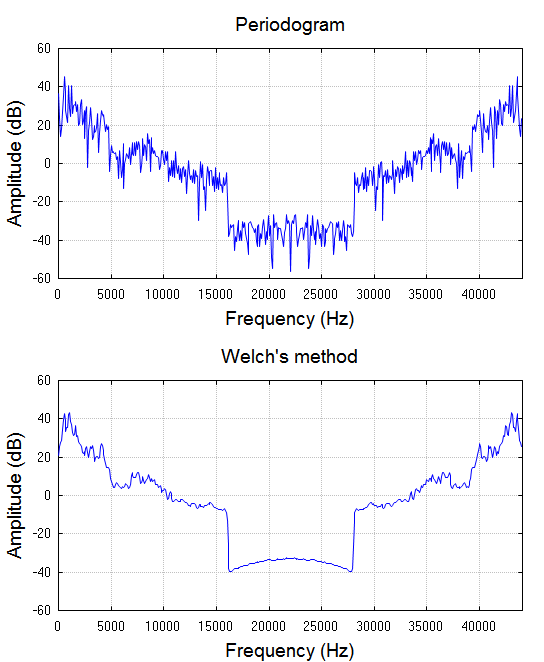
\includegraphics[height=3in]{Welch.png}}
    \end{block}
  \end{columns}
  \begin{tiny}
    Public domain image, 2016, Bob K,
    \url{https://commons.wikimedia.org/wiki/File:Comparison_of_periodogram_and_Welch_methods_of_spectral_density_estimation.png}\par
  \end{tiny}
\end{frame}

%%%%%%%%%%%%%%%%%%%%%%%%%%%%%%%%%%%%%%%%%%%%
\section[Summary]{Summary}
\setcounter{subsection}{1}

\begin{frame}
  \frametitle{Summary}
  \begin{itemize}
    \item Wiener Filter in the General Case:
      \begin{displaymath}
        H(\omega) =\frac{E\left[R_{sx}(\omega)\right]}{E\left[R_{xx}(\omega)\right]}
      \end{displaymath}
    \item Wiener Filter for Uncorrelated Noise:
      \begin{align*}
        H(\omega)
        &=\frac{E\left[R_{ss}(\omega)\right]}{E\left[R_{xx}(\omega)\right]}
      \end{align*}
    \item Welch's Method:
      chop the signal into frames, compute $|X(\omega)|^2$ for each frame, and then average them.
  \end{itemize}
\end{frame}

\end{document}
